\subsection{Other Circuits:}

The circuits in section 3.4 were simulated, and, as we can see, the behavior was exactly the same. For circuits in Figures 4.3.0 and 4.3.1, depending the semi-cycle in $V_{i}$, that is, if the semi-cycle it's in the positive region, the LED will be brighter, this because the transistor it's receiving voltage in the terminal of the base, in consequence, the voltage it's being empowered, same for current and analogously the power. \hfill \break

\begin{multicols}{2}
\begin{figure}[H]
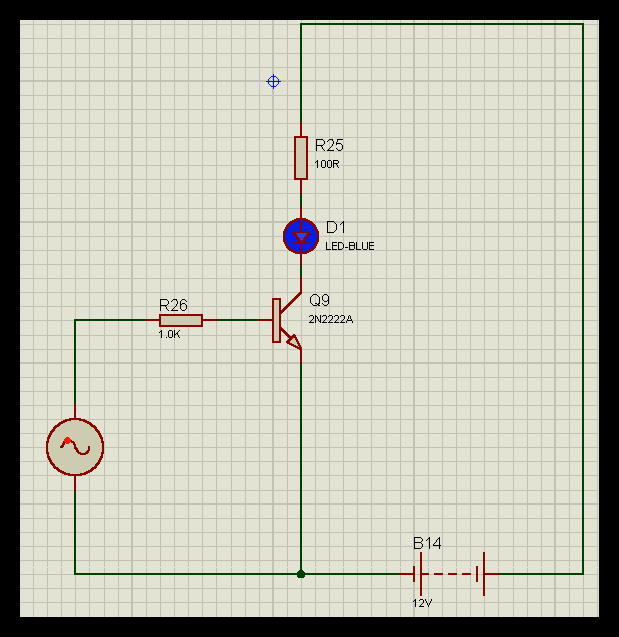
\includegraphics[scale=.35]{LED-On.png}
\centering \linebreak \linebreak Figure 4.3.0:  2N2222A - LED circuit when $V_{i}$ it's in the positive semi-cycle.
\end{figure}

\begin{figure}[H]
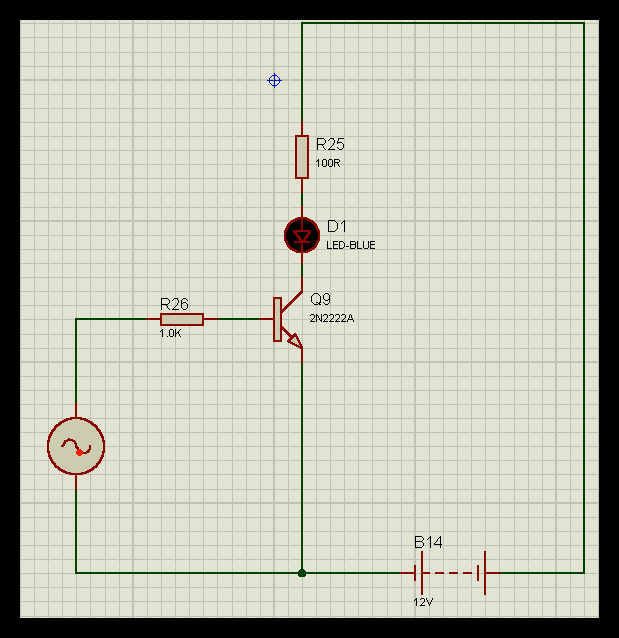
\includegraphics[scale=.35]{LED-Off.png}
\centering \linebreak \linebreak Figure 4.3.1: 2N2222A - LED circuit when $V_{i}$ it's in the negative semi-cycle.
\end{figure}
\end{multicols} \hfill

The same behavior we visualize in Figures 4.3.2 and 4.3.3, instead of using a LED, we are using a DC motor. When $V_{i}$ it's in the positive semi-cycle the speed in the {\bfseries RPM} display in the simulation increase, in the other case, when $V_{i}$ it's in the negative semi-cycle, the speed starts to slow down until $V_{i}$ reach its positive semi-cycle again. \hfill \break

\begin{multicols}{2}
\begin{figure}[H]
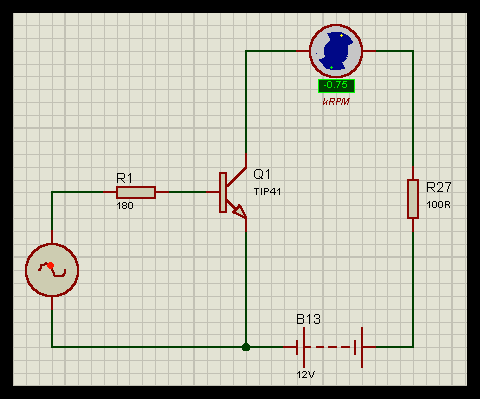
\includegraphics[scale=.45]{Motor-Positive-Semicycle.png}
\centering \linebreak \linebreak Figure 4.3.2:  TIP41 - Motor circuit when $V_{i}$ it's in the positive semi-cycle.
\end{figure}

\begin{figure}[H]
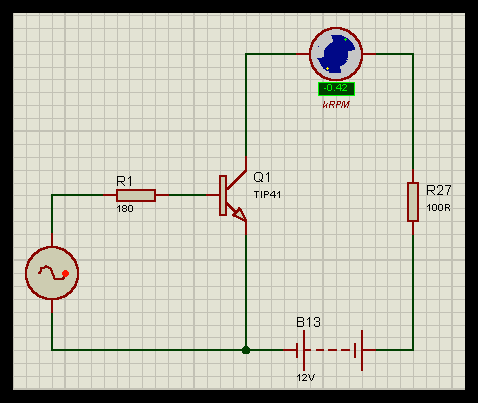
\includegraphics[scale=.45]{Motor-Negative-Semicycle.png}
\centering \linebreak \linebreak Figure 4.3.3: TIP41 - Motor circuit when $V_{i}$ it's in the negative semi-cycle.
\end{figure}
\end{multicols} \hfill

{\bfseries\itshape\color{carmine}{Observation:}} {\itshape\color{carmine}{In case that cannot be visualized, the {\bfseries RPM} display in Figure 4.3.2 it's up to 0.70, and in Figure 4.3.3 it's near to 0.40.}}

\pagebreak